\documentclass{TDP003mall}
\usepackage[utf8]{inputenc}
\usepackage[swedish]{babel}


\newcommand{\version}{Version 1.1}
\author{Daniel Huber, \url{danhu849@liu.se}\\
  Jens Öhnell, \url{jenoh242@liu.se}}
\title{Systemdokumentation}
\date{2020-10-21}
\rhead{Daniel Huber\\
Jens Öhnell}



\begin{document}
\projectpage
\section{Revisionshistorik}
\begin{table}[!h]
\begin{tabularx}{\linewidth}{|l|X|l|}
\hline
Ver. & Revisionsbeskrivning & Datum \\\hline
1.1 & Kompletterad Systemdokumentation TDP003 & 211020 \\\hline
1.0 & Systemdokumentation för Portfolio TDP003 & 151020 \\\hline
\end{tabularx}
\end{table}


\section{Översiktsbild}
Hemsidans syfte är att presentera information om hemsidans ägare, och presentera projekt som denna har gjort på ett sökbart sätt. Hemsidan byggs upp av ett datalager samt ett presentationslager.
\begin{figure}[h]
  \centerline{\includegraphics[width=\textwidth, height=10cm]{../Pictures/Översiktsbild.pdf}}
  \caption{Översiktsbild för portfolion. \label{fig:1}}
\end{figure}

\subsection{Datalagret}
I datalagret görs information om olika projekt åtkommlig och sökbar. Det skrevs i Python3 och projekten sparas i JSON i en JSON fil.

\subsection{Presentationslagret}
I presentationslagret görs informationen tillgänglig för slutanvändaren på ett enkelt och intuitivt sätt. Lagret skrevs i Python 3 med ramverket Flask samt templatemotorn Jinja2.

\section{Specifikation - Presentationslagret}
Skapandet av hemsidan har utgått från en kravspecifikation. Denna har varit vägledande i vilken funktionalitet sidan skall ha. Den fulla specifikationen kan hittas i dokumentet \textit{Systemspecifikation av portfoliosystem} som återfinns på kurshemsidan.

Sammanfattningsvis utgörs hemsidan av följande:
\begin{itemize}
    \item En förstasida med bilder.
    \item En söksida som gör det möjligt att söka och sortera på diverse fält för projekten.
    \item En tekniksida som gör det möjligt att sortera projekt på använda tekniker.
    \item Bilder, både "thumbnails" och fullstora, för alla projekt.
    \item För slutanvändaren begripliga felmedelanden.
    \item Korrekta statuskoder.
\end{itemize}

\newpage
\section{Sekvensdiagram - Sökning}

\begin{figure}[h]
  \centerline{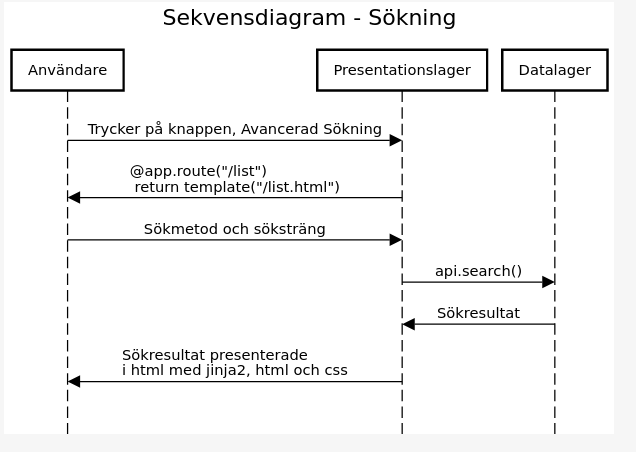
\includegraphics[width=\textwidth, height=10cm]{../Pictures/Sekvensdiagram.png}}
  \caption{Sekvensdiagram för Sökning \label{fig:2}}
\end{figure}

I sekvensdiagram \ref{fig:2} visas det översiktligt hur användaren från \texttt{(/home, /)} presenteras med sökresultat.

\section{Felhantering och Loggar}
Samtliga portfoliohändelser loggas med hjälp av Pythons \texttt{logging.config} modul. Konfigurationen för loggningen definieras i filen \texttt{logging.cfg}. Loggar skrevs till filen \texttt{portfolio\_log.log} i kronologisk ordning. Senast log längst ner. Båda filerna finns i root-katalogen för portfolio-appen. Loggar sparas med datumstämpel, viktighet, namn, tråd och meddelande. Alla loggar skrivs in i logfilen oavsett viktighet, men kan ändras vid behov genom att ändra \texttt{level=DEBUG} under \texttt{[logger\_root]} i konfigurationsfilen \texttt{logging.cfg}. En filtrationsnivå över \texttt{DEBUG} rekommenderas ej då händelser som lett upp till kraschen kan ha filtrerats bort. Logfilen finns tillgänglig även när \texttt{flask} inte körs. Vid ny körning av \texttt{flask} skrivs inte \texttt{portfolio\_log.log} över utan nya loggar skrivs in längst ner i filen.

Terminalkommandot tail med flaggan \texttt{-f} används vid \texttt{flask run} för att i realtid övervaka de senast tillagda loggarna i \texttt{portfolio\_log.log}. Vid behov används flaggan \texttt{nN} där \texttt{N} definieras av antalet rader som visas. Utan flaggan \texttt{-n} visas de sista 10 raderna från filen i terminalen. Att alltid de 10 sista raderna visas från filen möjliggörs av flaggan \texttt{-f}.

\texttt{tail -n15 -f /path/to/portfolio\_app/portfolio\_log.log}

Utöver logfilen hanteras fel med hjälp av Pythons \texttt{print()} funktion som kan skrivas in i varje \texttt{@app.route()} funktion, men också egendefinierade funktioner. Informationen skrivs ut i terminalfönstret när funktioner aktiveras under en flask run körning. Med \texttt{print()} kan variabler från bland annat databasen kommas åt. Flasks egen debug mode aktiveras genom att \texttt{FLASK\_DEBUG} variabeln sätts till 1 innan flask run:

\texttt{export FLASK\_DEBUG=1}

\subsection{Testning/felsökning - Databas}
Testning av datalagrets funktioner tillhandahålls av kursledningen och benämns enhetstester. Utöver de initiella enhetstesterna har fler med tiden lagts till. Enhetstesterna skrevs i Python3 där Pythons modul unittest (Unit testing framework) används. Testerna skrevs med kravspecifikationen i åtanke. Körning av testerna utan fel bevisar att funktionens krav uppfylls. Funktionerna för datalagret felsöks lättast med \texttt{print()} funktionen.

\section{Kod}
För fullständig dokumentation av kod, se dokumentet \textit{Portfoliodokumentation}.

\end{document}

%%% Local Variables:
%%% mode: latex
%%% TeX-master: t
%%% End:
